\subsection{Klassenzimmer als Eye-Tracking Umgebung}
\begin{frame}
\begin{center}
	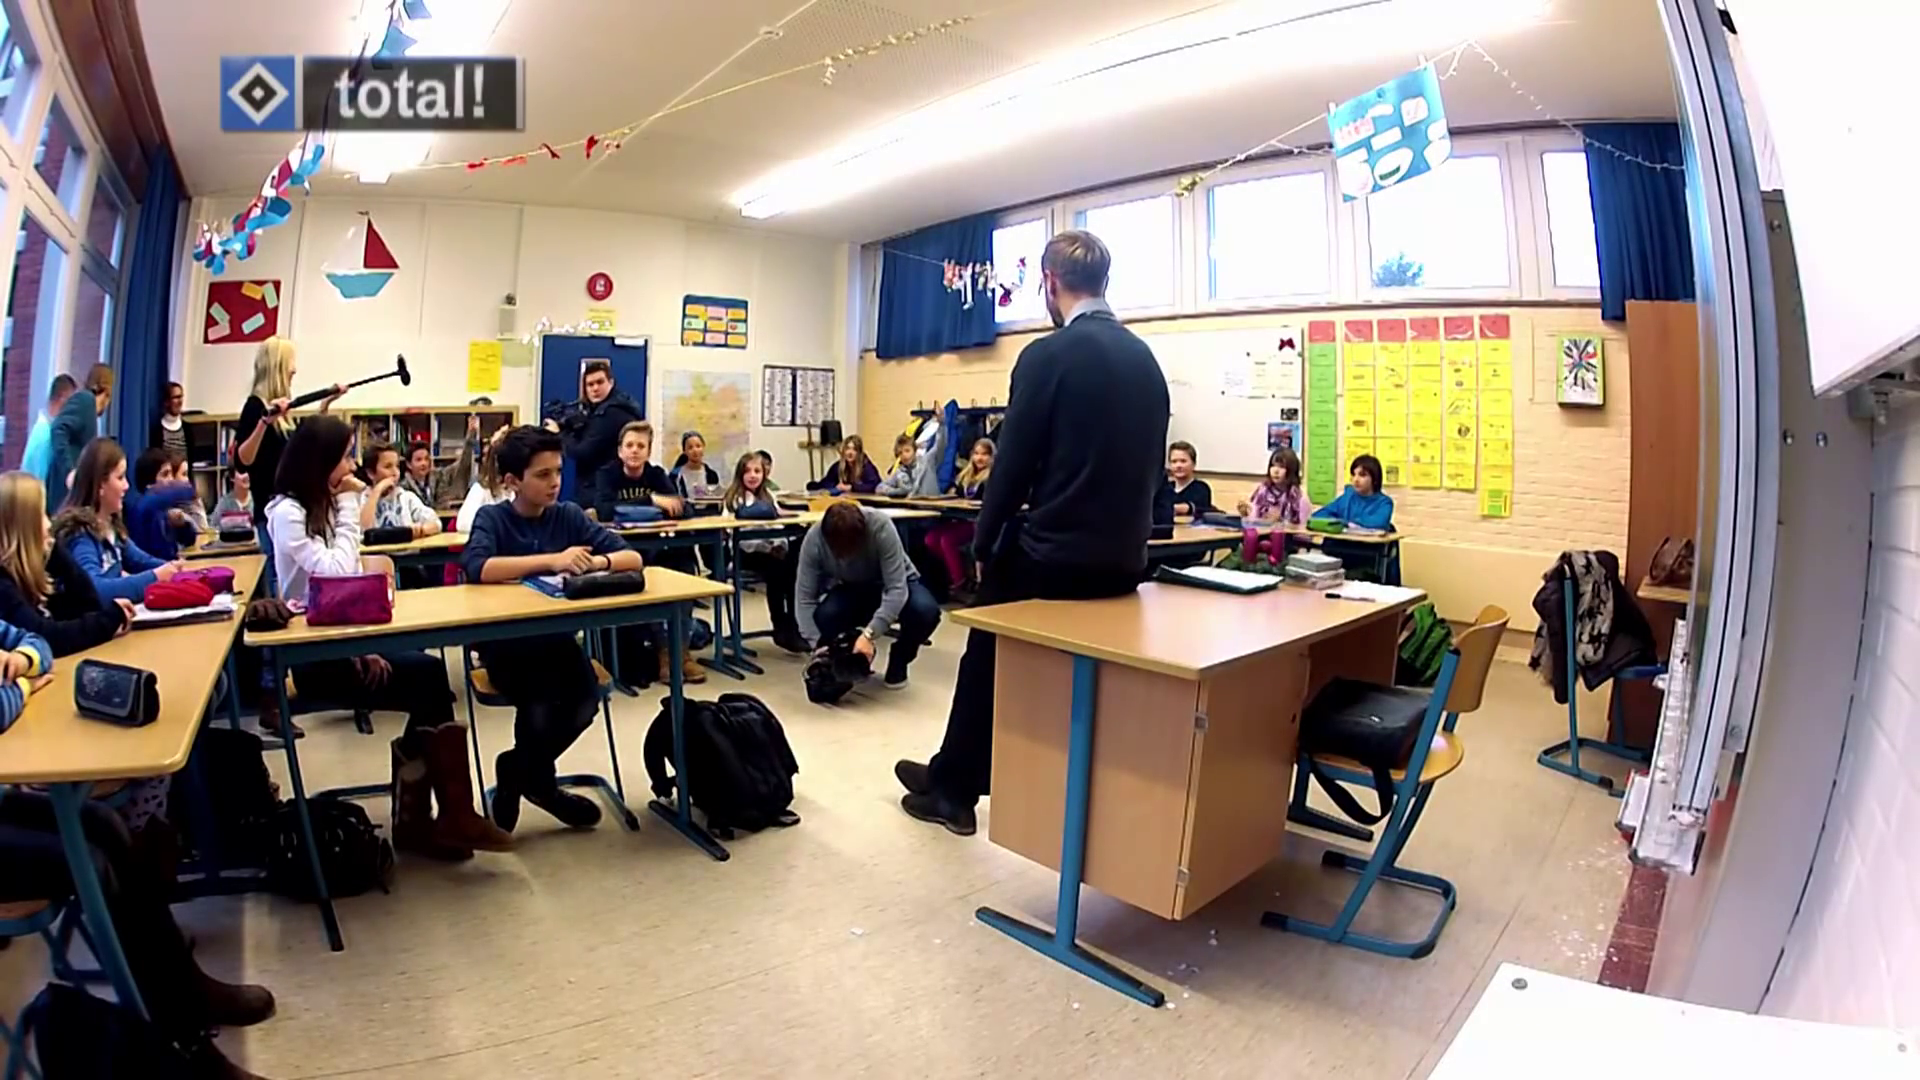
\includegraphics[width=0.55\linewidth]{images/Schulklasse}
\end{center}
\begin{itemize}
	\item<1-> Blickrichtung und Gesichtsorientierung der Schüler sollen so exakt wie möglich erfasst werden.
	\item<1-> Das Verfahren muss gleichzeitig auf $2,5 - 8m$ bei einer Breite von $6m$ funktionieren.\\
	Klassenzimmer: $54-66m^2$ für max. $31$ Schüler
	\item<1-> Der Unterricht soll durch die Aufnahme möglichst wenig gestört werden
	\item<1-> Die Aufnahme der Schulklasse erfolgt innerhalb eines Gebäudes
\end{itemize}
\end{frame}